\subsection{Address Translation}
\label{sec:paging}

% Outcome: understanding the isolation provided by address translation

System software relies on the CPU's address translation mechanism for
implementing isolation among less privileged pieces of software (applications
or operating systems). Virtually all secure architecture designs bring changes
to address translation. We summarize the Intel architecture's address
translation features that are most relevant when establishing a system's
security properties, and refer the reader to \cite{jacob1998virtual} for a more
general presentation of address translation concepts and its other uses.


\subsubsection{Address Translation Concepts}

From a systems perspective, address translation is a layer of indirection
(shown in Figure~\ref{fig:address_translation}) between the
\textit{virtual addresses}, which are used by a program's memory load and store
instructions, and the \textit{physical addresses}, which reference the physical
address space (\S~\ref{sec:address_spaces}). The mapping between virtual and
physical addresses is defined by \textit{page tables}, which are managed by the
system software.

\begin{figure}[hbt]
  \centering
  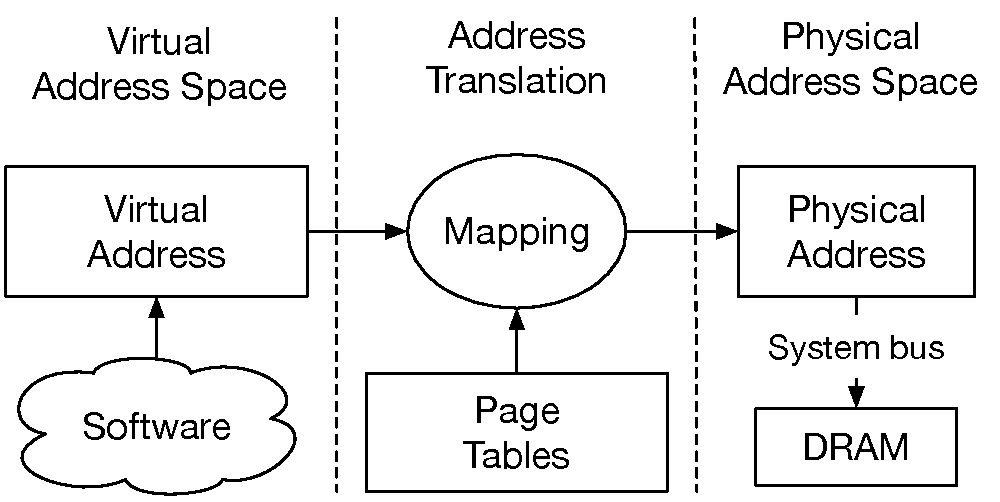
\includegraphics[width=75mm]{figures/address_translation.pdf}
  \caption{
    Virtual addresses used by software are translated into physical memory
    addresses using a mapping defined by the page tables.
  }
  \label{fig:address_translation}
\end{figure}

Operating systems use address translation to implement the \textit{virtual
memory} abstraction, illustrated by Figure~\ref{fig:virtual_memory}, which
gives each process its own virtual address space that acts as if the process
owned the entire computer's memory.

\begin{figure}[hbt]
  \centering
  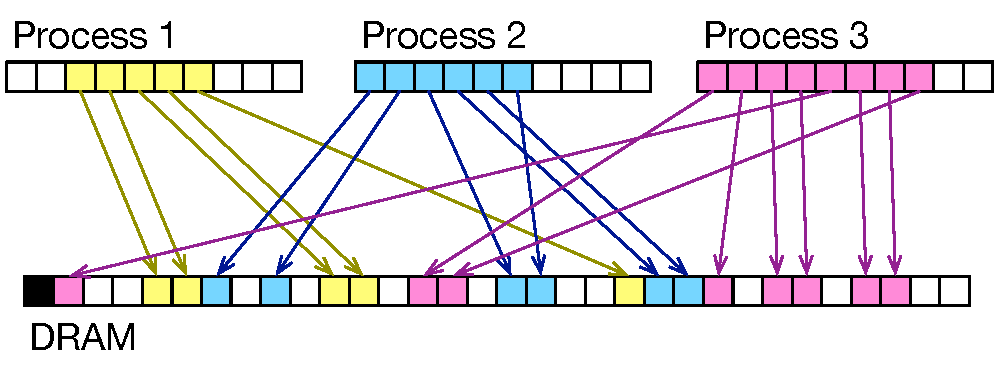
\includegraphics[width=80mm]{figures/virtual_memory.pdf}
  \caption{
    The virtual memory abstraction gives each process its own virtual address
    space. The operating system multiplexes the computer's DRAM between the
    processes, while application developers build software as if it owns the
    entire computer's memory.
  }
  \label{fig:virtual_memory}
\end{figure}

Address translation is used by the operating system to multiplex DRAM among
multiple application processes, isolate the processes from each other, and
prevent application code from accessing memory-mapped devices directly. The
latter two protection measures prevent an application's bugs from impacting
other applications or the OS kernel itself. Hypervisors also use address
translation, to divide the DRAM among operating systems that run concurrently,
and to virtualize memory-mapped devices.

% Canonical Addressing: SDM vol1 S 3.3.7.1
% IA-32e Paging: SDM S 4.5

The address translation mode used by 64-bit operating systems, called
IA-32e by Intel's documentation, maps 48-bit \textit{virtual addresses} to
\textit{physical addresses} of at most 52 bits\footnote{The size of a
physical address is CPU-dependent, and is 40 bits for recent desktop CPUs and
44 bits for recent high-end server CPUs.}. The translation process, illustrated
in Figure~\ref{fig:os_paging}, is carried out by dedicated hardware in the CPU,
which is referred to as the \textit{address translation unit} or the
\textit{memory management unit} (MMU).

\begin{figure}[hbt]
  \centering
  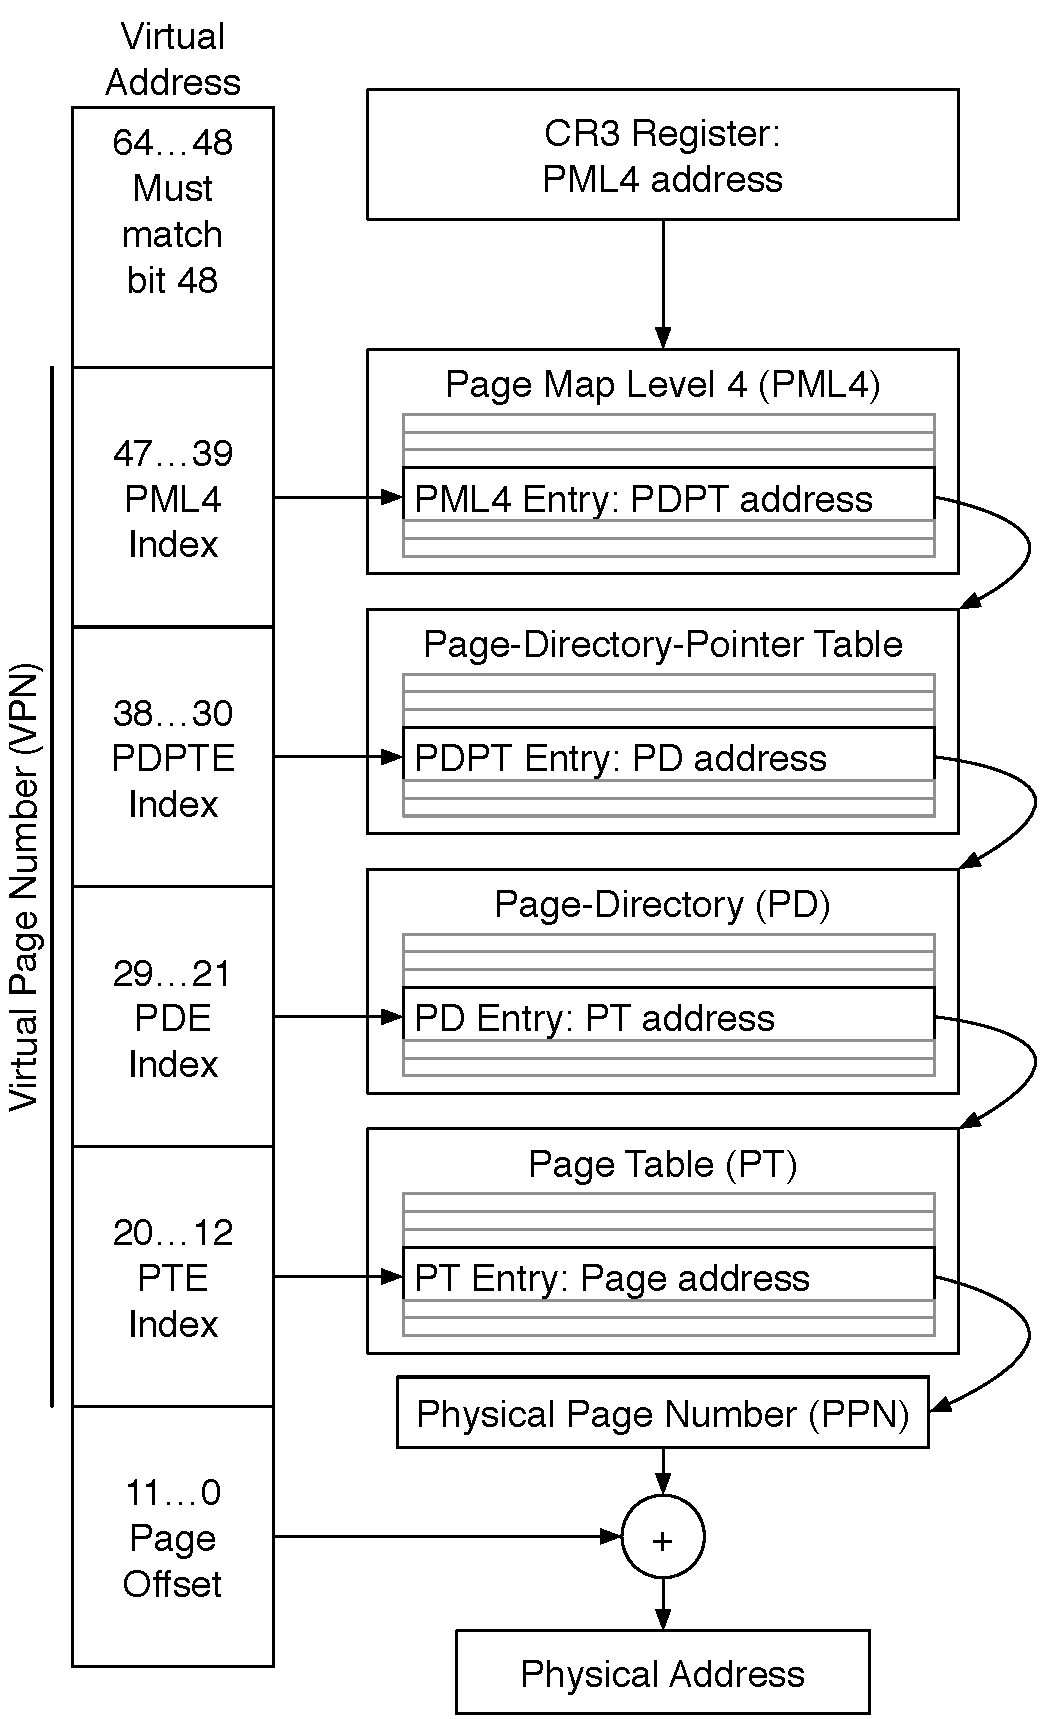
\includegraphics[width=85mm]{figures/os_paging.pdf}
  \caption{
    IA-32e address translation takes in a 48-bit virtual address and outputs
    a 52-bit physical address.
  }
  \label{fig:os_paging}
\end{figure}

The bottom 12 bits of a virtual address are not changed by the translation. The
top 36 bits are grouped into four 9-bit indexes, which are used to index into
the page tables. Despite its name, the page tables data structure closely
resembles a full 512-ary search tree where nodes have fixed keys. Each
node is represented in DRAM as an array of 512 8-byte entries that contain the
physical addresses of the next-level children as well as some flags. The
physical address of the root node is stored in the CR3 register. The arrays in
the last-level nodes contain the physical addresses that are the result of the
address translation.

The address translation function, which does not change the bottom bits of
addresses, partitions the memory address space into \textit{pages}. A page is
the set of all memory locations that only differ in the bottom bits which are
not impacted by address translation, so all the memory addresses in a virtual
page translate to corresponding addresses in the same physical page. From this
perspective, the address translation function can be seen as a mapping between
\textit{Virtual Page Numbers} (VPN) and \textit{Physical Page Numbers} (PPN),
as shown in Figure~\ref{fig:address_translation_bits}.

\begin{figure}[hbt]
  \centering
  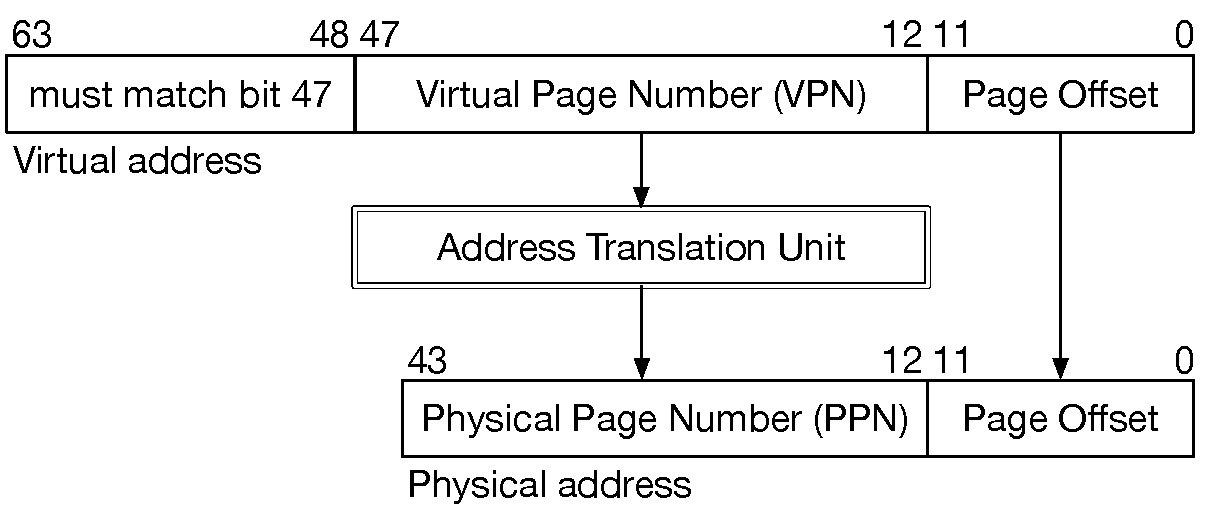
\includegraphics[width=85mm]{figures/address_translation_bits.pdf}
  \caption{
    Address translation can be seen as a mapping between virtual page numbers
    and physical page numbers.
  }
  \label{fig:address_translation_bits}
\end{figure}

In addition to isolating application processes, operating systems also use the
address translation feature to run applications whose collective memory
demands exceed the amount of DRAM installed in the computer. The OS evicts
infrequently used memory pages from DRAM to a larger (but slower) memory, such
as a hard disk drive (HDD) or solid-state drive (SSD).

The OS ability to over-commit DRAM is often called \textit{page swapping}, for
the following reason. When an application process attempts to access a page
that has been evicted, the OS ``steps in'' and reads the missing page back into
DRAM. In order to do this, the OS might have to evict a different page from
DRAM, effectively swapping the contents of a page in DRAM with a page in the
slower memory. The details behind this high-level description are covered in
the following sections.

The CPU's address translation is also referred to as ``paging'', which is a
shorthand for ``page swapping''.


\subsubsection{Address Translation and Virtualization}
\label{sec:vmx_paging}

% VMX Support for Address Translation: SDM S 4.11

Computers that take advantage of hardware virtualization use a hypervisor to
run multiple operating systems at the same time. This creates some tension,
because each operating system was written under the assumption that it owns the
entire computer's DRAM. The tension is solved by a second layer of address
translation, illustrated in Figure~\ref{fig:vmx_address_translation}.

\begin{figure}[hbt]
  \centering
  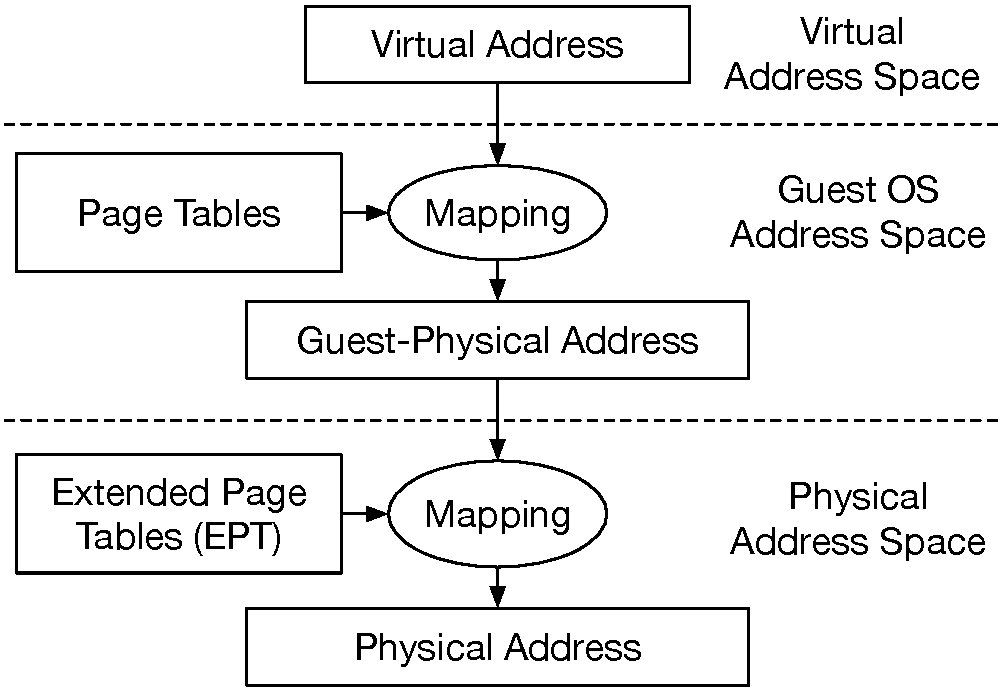
\includegraphics[width=70mm]{figures/vmx_address_translation.pdf}
  \caption{
    Virtual addresses used by software are translated into physical memory
    addresses using a mapping defined by the page tables.
  }
  \label{fig:vmx_address_translation}
\end{figure}


When a hypervisor is active, the page tables set up by an operating system map
between virtual addresses and \textit{guest-physical addresses} in a
\textit{guest-physical address space}. The hypervisor multiplexes the
computer's DRAM between the operating systems' guest-physical address spaces
via the second layer of address translations, which uses \textit{extended page
tables}~(EPT) to map guest-physical addresses to physical addresses.

The EPT uses the same data structure as the page tables, so the process of
translating guest-physical addresses to physical addresses follows the same
steps as IA-32e address translation. The main difference is that the physical
address of the data structure's root node is stored in the extended page table
pointer~(EPTP) field in the \textit{Virtual Machine Control Structure}~(VMCS)
for the guest OS. Figure~\ref{fig:vmx_paging} illustrates the address
translation process in the presence of hardware virtualization.

\begin{figure}[hbt]
  \centering
  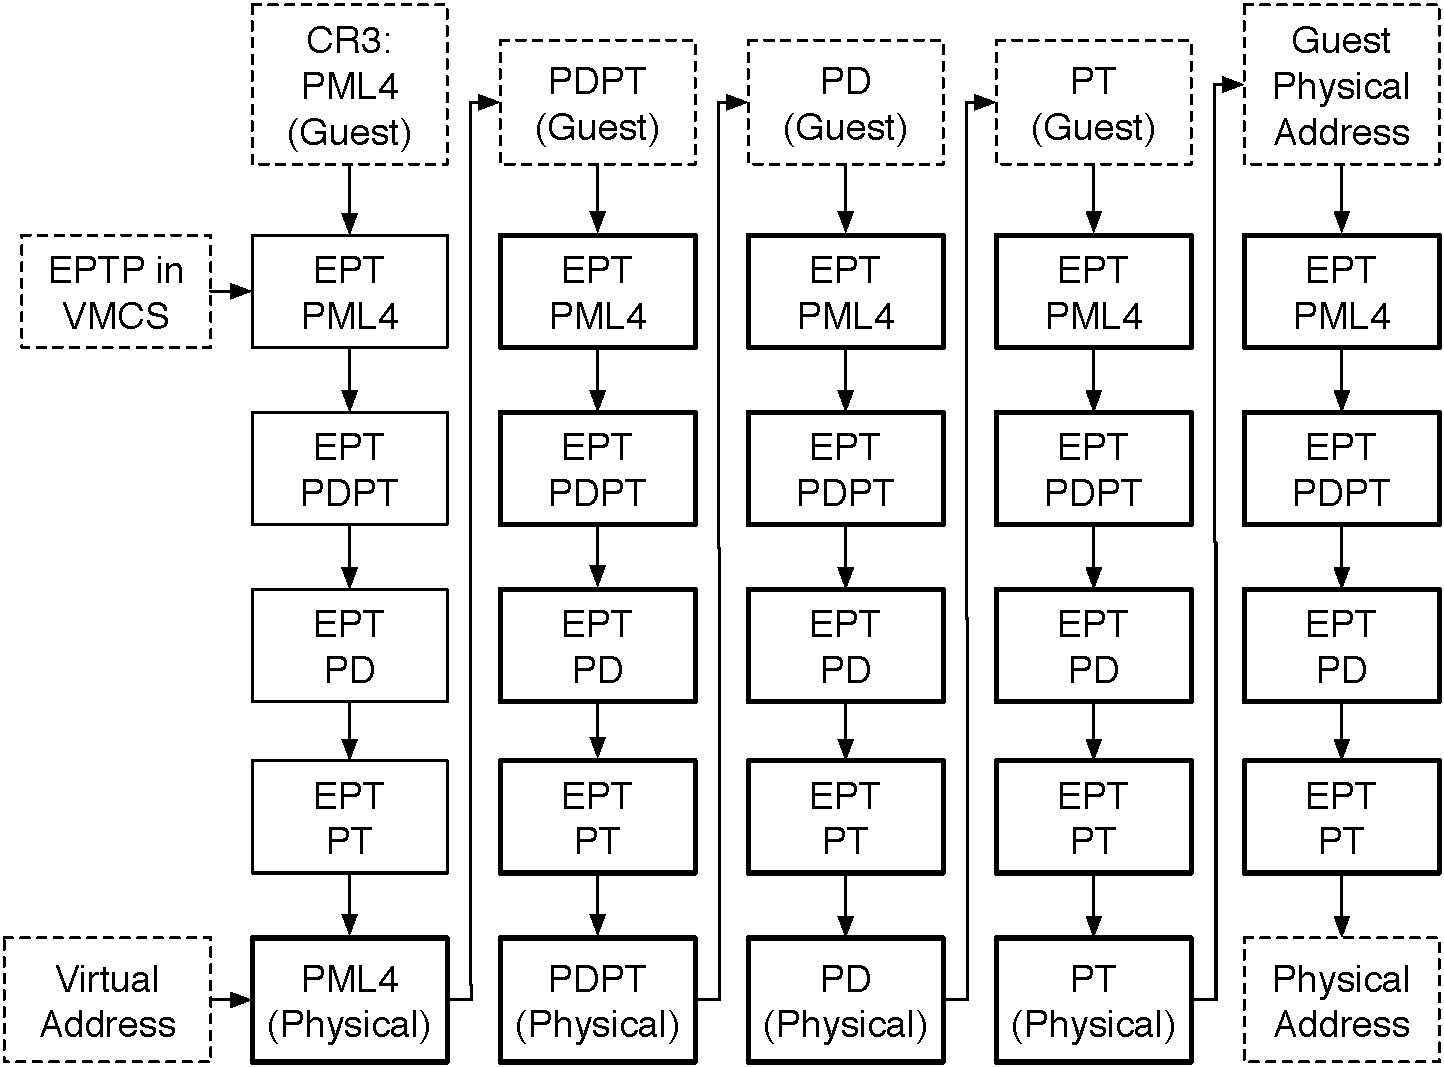
\includegraphics[width=85mm]{figures/vmx_paging.pdf}
  \caption{
    Address translation when hardware virtualization is enabled. The
    kernel-managed page tables contain guest-physical addresses, so each level
    in the kernel's page table requires a full walk of the hypervisor's
    extended page table~(EPT).  A translation requires up to 20 memory accesses
    (the bold boxes), assuming the physical address of the kernel's PML4 is
    cached.
  }
  \label{fig:vmx_paging}
\end{figure}


\subsubsection{Page Table Attributes}
\label{sec:page_table_attributes}

Each page table entry contains a physical address, as shown in
Figure~\ref{fig:os_paging}, and some Boolean values that are referred to as
\textit{flags} or \textit{attributes}. The following attributes are used to
implement page swapping and software isolation.

The \textit{present}~(P) flag is set to 0 to indicate unused parts
of the address space, which do not have physical memory associated with them.
The system software also sets the P flag to 0 for pages that are evicted from
DRAM. When the address translation unit encounters a zero P flag, it aborts the
translation process and issues a hardware exception, as described in
\S~\ref{sec:faults}. This hardware exception gives system software an
opportunity to step in and bring an evicted page back into DRAM.

The \textit{accessed}~(A) flag is set to 1 by the CPU whenever the address
translation machinery reads a page table entry, and the \textit{dirty}~(D) flag
is set to 1 by the CPU when an entry is accessed by a memory write operation.
The A and D flags give the hypervisor and kernel insight into application
memory access patterns and inform the algorithms that select the pages that get
evicted from RAM.

% Page-Level Protection: SDM S 5.11, S 5.11.{1,2,3,4}

The main attributes supporting software isolation are the
\textit{writable}~(W) flag, which can be set to 0 to
prohibit\footnote{Writes to non-writable pages result in \#GP exceptions
(\S~\ref{sec:faults}).} writes to any memory location inside a page, the
\textit{disable execution}~(XD) flag, which can be set to 1 to prevent
instruction fetches from a page, and the \textit{supervisor}~(S) flag, which
can be set to 1 to prohibit any accesses from application software running at
ring 3.
